\documentclass[12pt]{article}%
\usepackage[a4paper, top=2.5cm, bottom=2.5cm, left=2.2cm, right=2.2cm]
{geometry}
\usepackage{float}
\usepackage{graphicx}
\usepackage{listings}
\restylefloat{table}

%---------------------------------------------------------------------------
\begin{document}
\title{Switcher}
\author{Ashley J. Robinson}
\date{\today}
\maketitle
%---------------------------------------------------------------------------
\section{Introduction}


\section{Hardware}


\section{Software}

\subsection{Peripherals}

\subsubsection{Analogue to Digital Convertors (ADCs)}

A single ADC is multiplexed to measure three voltages on the board. 

\subsubsection{Universal Asyncronhouse/Syncronhous Transceiver (UART)}

The UART is configure to run at 115200 baud with no control flow with a ring buffer interface. Trasmission from the microcontroller happens through \textbf{uartLoadOut} which adds to the \textbf{8 byte} buffer and is then unloaded from a timer. The input is not interrupt driven and is handled in the main control loop using a \textbf{5 byte} buffer that is enough to contain the longest command.

\subsubsection{Programmable Counter Array (PCA)}

The Pulse Width Modulation (PWM) is controlled from the counter array. The output runs at approximatly 96KHz with 8 bits to control the duty cycle. A high resolution for control would be favourable for this application but the frequency achieved in 16-bit mode is far too low for this application.

\subsubsection{Timers}

\textbf{Timer 0} is used as baud rate generagtion for the UART. \textbf{Timer 2} is used to trigger an Interrupt Service Routine (ISR) which runs at 4KHz. The ISR control the UART transmission, sampling of the ADC, running the controller and finally setting the PWM.

\subsection{Operation}

\begin{figure}[H]
	\centering
  	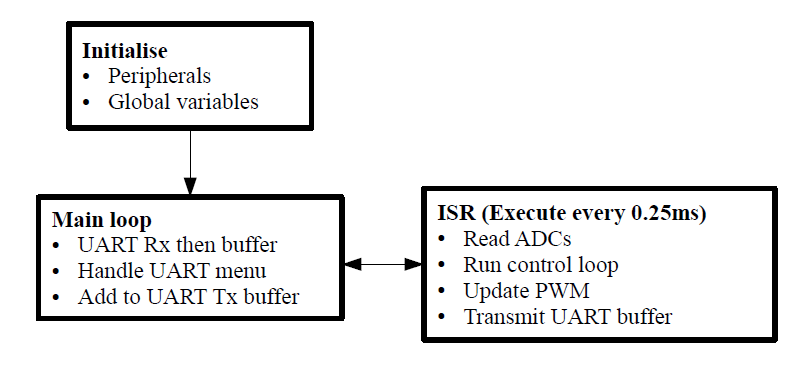
\includegraphics[width=12cm]{code.png}
  	\caption{Software overview.}
  	\label{fig:overview}
\end{figure}



\subsection{UART Menu}
\begin{table}[H]
   \centering
   \caption{UART menu}
   \label{tab:menu}
   \begin{tabular}{|p{4cm}|p{1.2cm}|p{1.8cm}|p{1.8cm}|p{4cm}|}
   \hline
      \textbf{Command}              & \textbf{Char}   &  \textbf{Send numbers}   &  \textbf{Return numbers}  &  \textbf{Notes}\\ \hline
      Enable                        & g               &  0                       &  0                        &  0                        \\ \hline
      Disable                       & s               &  0                       &  0                        &  0                        \\ \hline
      Read ADC1                     & x               &  0                       &  4                        &  Result in mV                         \\ \hline
      Read ADC2                     & y               &  0                       &  4                        &  Result in mV                         \\ \hline
      Read ADC3                     & z               &  0                       &  4                        &  Result in mV                         \\ \hline
      Read output current           & j               &  0                       &  4                        &  Result in mA              \\ \hline
      Set output voltage            & v               &  4                       &  0                        &  Send value in mV         \\ \hline
      Set otuput current            & c               &  4                       &  0                        &  Send value in mA    \\ \hline
      Set controller P              & p               &  4                       &  0                        &  Value is divide by 10    \\ \hline
      Set controller I              & i               &  4                       &  0                        &  Value is divide by 10         \\ \hline
      Set input voltage upper limit & u               &  4                       &  0                        &  Send value in mV             \\ \hline
      Set input voltage lower limit & l               &  4                       &  0                        &  Send value in mV         \\ \hline
   \end{tabular}
\end{table}



\subsection{Assembly analysis}

The following sections of code are library function inserted by the compilier implict to facilite some more complex operations.

\subsubsection{ADC scaling}

Listing \ref{adc0} is a line of code operating on a 32 bit signed integer and invokes listing \ref{limul} and \ref{ulshr}. The purpose of this operation is to cast the voltage recorded by the ADC to a representation in mV. It is possible for the target voltage to be translated instead but this would still require the same piece of code. The 12 bit oputput but the ADC must be multiplied 5.926 as to represent the voltage at the top of the potential divider. Fixed but multiplication followed by a shift operation removes the need for a floating point operation but yeilds the same result.

\lstset{
  caption=LIMUL, 
  basicstyle=\footnotesize, frame=tb,basicstyle=\fontsize{6}{7}\ttfamily,
  xleftmargin=.2\textwidth, xrightmargin=.2\textwidth,
label=adc0
}
\begin{lstlisting}
return (((U32)ADC0)*SCALE_MUL) >> 10;
\end{lstlisting}




\subsubsection{ADC scaling}






\subsubsection{Division}

Division and modulus operations are contained in \ref{div} invoke the functions contained in \ref{udiv}.

\lstset{
  caption=Division, 
  basicstyle=\footnotesize, frame=tb,basicstyle=\fontsize{6}{7}\ttfamily,
  xleftmargin=.2\textwidth, xrightmargin=.2\textwidth,
label=div
}
\begin{lstlisting}
scale /= 10;

num = out / scale;

out %= scale;	
\end{lstlisting}


\subsubsection{Switch}

This library function is generated to control large switch statements??

\section{Conclusion}

The complete assembly in listing \ref{switcher.asm} is generated from the code in listing \ref{main.c}. The C code is contained within a single file and generates $950$ lines of assembler with an additional $3$ lines contained within the jump table and the jump on reset...

\begin{itemize}
  	\item \textbf{0x0000} Jumps straight to 0x0800
	\item \textbf{0x001B} Jump table entry TIMER1\_ISR(C:0BB6)
	\item \textbf{0x002B} Jump table entry TIMER2\_ISR(C:094C)
	\item \textbf{0x0800} First line of code generated from main.c
  	\item \textbf{0x0BB6} Final line of code generated from main.c
\end{itemize}

The Keil c51 compilier limits machine code generation to 2KB (not a problem) however it also limits the use of memory less than 2KB by always jumping to address $2048$ and then continuing with the compiled assembler. Excluding the first $2048$ is not completely fair because the jump on reset and the jump table would still exsist. The highest vector used in the jump table is at address $43$ so assuming this is not optimised by the compilier the total code size comes to \textbf{993 bytes}.

\section{Appendix}

\subsection{Code listings}

\lstset{
  caption=main.c, 
  basicstyle=\fontsize{6}{7}\ttfamily, frame=tb,
  xleftmargin=.05\textwidth, xrightmargin=.05\textwidth,
label=main.c, tabsize=4	
}
\lstinputlisting[language=C]{main.c}

\lstset{
  caption=Swicther.asm, 
  basicstyle=\footnotesize, frame=tb,basicstyle=\fontsize{6}{7}\ttfamily,
  xleftmargin=.2\textwidth, xrightmargin=.2\textwidth,
label=switcher.asm
}
\lstinputlisting{Switcher.asm}

\lstset{
  caption=LIMUL, 
  basicstyle=\footnotesize, frame=tb,basicstyle=\fontsize{6}{7}\ttfamily,
  xleftmargin=.2\textwidth, xrightmargin=.2\textwidth,
label=limul
}
\lstinputlisting{limul.asm}

\lstset{
  caption=ULSHR, 
  basicstyle=\footnotesize, frame=tb,basicstyle=\fontsize{6}{7}\ttfamily,
  xleftmargin=.2\textwidth, xrightmargin=.2\textwidth,
label=ulshr
}
\lstinputlisting{ulshr.asm}


\lstset{
  caption=IMUL, 
  basicstyle=\footnotesize, frame=tb,basicstyle=\fontsize{6}{7}\ttfamily,
  xleftmargin=.2\textwidth, xrightmargin=.2\textwidth,
label=imul
}
\lstinputlisting{imul.asm}


\lstset{
  caption=UDIV, 
  basicstyle=\footnotesize, frame=tb,basicstyle=\fontsize{6}{7}\ttfamily,
  xleftmargin=.2\textwidth, xrightmargin=.2\textwidth,
label=udiv
}
\lstinputlisting{udiv.asm}


\lstset{
  caption=CCASE, 
  basicstyle=\footnotesize, frame=tb,basicstyle=\fontsize{6}{7}\ttfamily,
  xleftmargin=.2\textwidth, xrightmargin=.2\textwidth,
label=ccase
}
\lstinputlisting{ccase.asm}



       
%---------------------------------------------------------------------------
\end{document}
